\documentclass[11pt]{sdm}
\usepackage{graphicx} % For figures
\usepackage{mathtools} % For smallmatrix envs
\usepackage{caption} % For figures captions
\usepackage{amsfonts} % For black board letters
\usepackage{bbm} % For black board 1
\usepackage[style=authoryear-comp, sorting=nyt, backend=biber]{biblatex} % For bibliography
\addbibresource{Biblio.bib}


\makeatletter

\newrobustcmd*{\parentexttrack}[1]{%
    \begingroup
    \blx@blxinit
    \blx@setsfcodes
    \blx@bibopenparen#1\blx@bibcloseparen
    \endgroup
}

\AtEveryCite{%
    \let\parentext=\parentexttrack%
    \let\bibopenparen=\bibopenbracket%
    \let\bibcloseparen=\bibclosebracket
}

\makeatother

%numeroter les pages
\pagestyle{plain}

\title{SCARE for Hardware SPN}
\author{Paul \textsc{Saurou}}
\supervisorOne{Benoît \textsc{Gérard}}
\supervisorTwo{Margaux \textsc{Dugardin}}
\team{SDCyb1/EPOC/XCS}
%One of:
% ens-Rennes  esir    insa-rennes   rennes1  
% enssat    logoUbs   tsupelec
%here rennes1 for example
\school{supelec}


% the domain should be one or two of:
% Technology for Human Learning 
% Artificial Intelligence 
% Computer Arithmetic
% Hardware Architecture
% Automatic Control Engineering
% Bioinformatics 
% Biotechnology
% Computational Complexity 
% Computational Engineering, Finance, and Science
% Computational Geometry 
% Computation and Language 
% Cryptography and Security 
% Computer Vision and Pattern Recognition
% Computers and Society 
% Databases 
% Distributed, Parallel, and Cluster Computing 
% Digital Libraries
% Discrete Mathematics 
% Data Structures and Algorithms 
% Embedded Systems 
% Emerging Technologies 
% Formal Languages and Automata Theory 
% General Literature 
% Graphics 
% Computer Science and Game Theory 
% Human-Computer Interaction 
% Computer Aided Engineering 
% Medical Imaging 
% Information Retrieval 
% Information Theory 
% Ubiquitous Computing 
% Machine Learning
% Logic in Computer Science 
% Multiagent Systems 
% Mobile Computing
% Multimedia
% Modeling and Simulation 
% Mathematical Software 
% Numerical Analysis 
% Neural and Evolutionary Computing 
% Networking and Internet Architecture 
% Operating Systems 
% Performance 
% Programming Languages 
% Robotics 
% Operations Research
% Symbolic Computation 
% Sound
% Software Engineering 
% Social and Information Networks 
% Systems and Control 
% Image Processing 
% Signal and Image Processing 
% Document and Text Processing
% Web
\domain{Domain: Cryptography and Security}

%write your abstract here
\abstract{write your abstract here}



\begin{document}
\maketitle

%*****************************************************************%

\section*{Introduction}

Following Kerckhoffs' principle, the security of a cryptographic device shall not rely on the secrecy of its mechanisms \parencite{Kerckhoffs_1883}.
However, in some specific contexts, having a secret implementation can add a layer of security, by increasing the practical difficulty of the attack.

\section{State of the art of Side Channel Attacks on SPNs}

In this section, we formally define substitution–permutation network ciphers.
Then, we introduce some of the most classical and standardized implementations.
Finally, we present several Side Channel Analysis classic attacks on these implementations.

\subsection{SPNs, Feistel schemes, DES and AES}

Symmetric cryptography refers to the protection of a communication between a sender and a receiver who share the same secret key.
An algorithm that derives from symmetric cryptography is called a symmetric algorithm.
Symmetric algorithms mostly rely on either substitution ciphers, stream ciphers or block ciphers.

\textbf{Substitution ciphers} replace the units of plaintext by ciphertext in a defined manner, with the help of a key.
Those are well known in history but can nowadays be easily decrypted using a frequency table or a similar mechanism.

\textbf{Stream ciphers} encrypt the characters (in the form of bytes) of a message one at a time.

\textbf{Block ciphers} encrypt fixed-length blocks of plaintext.

This internship will focus on block ciphers, and especially on substitution–permutation networks.

\subsubsection{Block ciphers}

A block cipher consists of both an encryption function $E$ and a decryption function $D=E^{-1}$.
They both accept two inputs: a block of text of fixed size $n$ and a key of size $k$.
They output a block of size $n$.

The difference between different block ciphers is the definition of the function $E$ (and $D$).

Most block ciphers are iterated, which means that $E$ consists in the repetition of a round function $R$ taking a different round key $K_i$ each round $i$ and the output of the previous round as the new input.
If $M_0$ is the plaintext and there are $r$ rounds, then $ \forall i \in [ 1,r ] , M_i = R(M_{i-1},K_i) $ and $M_r = E(M_0)$ is the ciphertext.
$R(M,K_i)$ is generally written $R_{K_i}(M)$.

Choosing the number of rounds of an iterated block cipher scheme is a compromise between computing efficiency, cryptographic security and side channels leakages.
Too few rounds allow for cryptographic attacks and too many rounds make the cipher inefficient and more difficult to implement securely.

We will now define two types of iterated block ciphers: Feistel networks and substitution–permutation networks.

\subsubsection{Feistel ciphers}

In a Feistel scheme, the plaintext block is divided in two parts $(p,q)$ of equal length $n/2$.
With the previous notations, the round function is $R: (p,q) \mapsto (q,p \bigoplus f(q,K_i))$ where $f$ is called the Feistel function.
Both the security and the performance of the Feistel network depend on the Feistel function $f$.
A specificity of Feistel schemes is that $f$ does not need to be invertible.
The decryption is almost identical to the encryption, the only difference being the reversal of the round keys order.

% TODO: add image

\subsubsection{DES}

The Data Encryption Standard (DES) is a Feistel network scheme that has been highly influential in the advancement of cryptography.
It is unsecure due to its too short 56-bit key size which make it vulnerable to brute-force attacks.
For historical reasons this design still is interesting.
It consists in a 16 round Feistel network and operates on blocks of 64 bits.
The Feistel function of DES is shown on %TODO: figure

First the 32-bit half-block is expanded to 48 bits using the $E$ expansion permutation function.
Then the 48-bit block is xored with the round subkey and goes through a substitution layer.
It is divided into eight 6-bit words which are replaced by 4-bit words using a lookup table.
Finally, the 32 outputs are mixed according to a fixed permutation, the P-box.


\subsubsection{SPN ciphers}

In substitution–permutation networks (SPN), the round function consists of a substitution stage followed by a permutation stage.
It splits the plaintext $M$ of size $n$ into $l$ blocks $m_1,m_2,...,m_l$ of equal length.
The substitution stage is non-linear and mixes the round key with the plaintext.
It uses a set of substitution-boxes (S-boxes) that do one-to-one substitution to be reversible.
The permutation stage rearranges all the bits of the output of the S-boxes each round, as shown on Figure \ref{fig_spn}.

More formally and with the previous notations, the round function is $R_{K_i} = \lambda \circ \gamma \circ \sigma_{K_i}$ with
\begin{itemize}
    \item $\sigma_{K}:M \mapsto M \bigoplus K$ the key addition layer,
    \item $\gamma : M=(m_1,m_2,...,m_l) \mapsto S_1(m_1),S_2(m_2),...,S_l(m_l)$ the substitution layer, where $(S_i)_{1\leq i \leq l}$ are non-linear substitution functions.
    \item $\lambda : M \mapsto A \times M$ the linear layer, where $\times$ is the matrix product.
\end{itemize}

In some SPN implementations, the final round sometimes skips the linear layer and an additional key addition is often performed after the final substitution layer.

The S-boxes $(S_i)_{1\leq i \leq l}$ can be chosen identical. 
All the S-boxes do not have the same cryptographic properties.
One is considered secure if it exhibits the avalanche effect, meaning that changing a small change in the input changes the output greatly.
For example, one input bit should change almost half of the output bits on average.
% TODO: Decryption

\begin{center}
    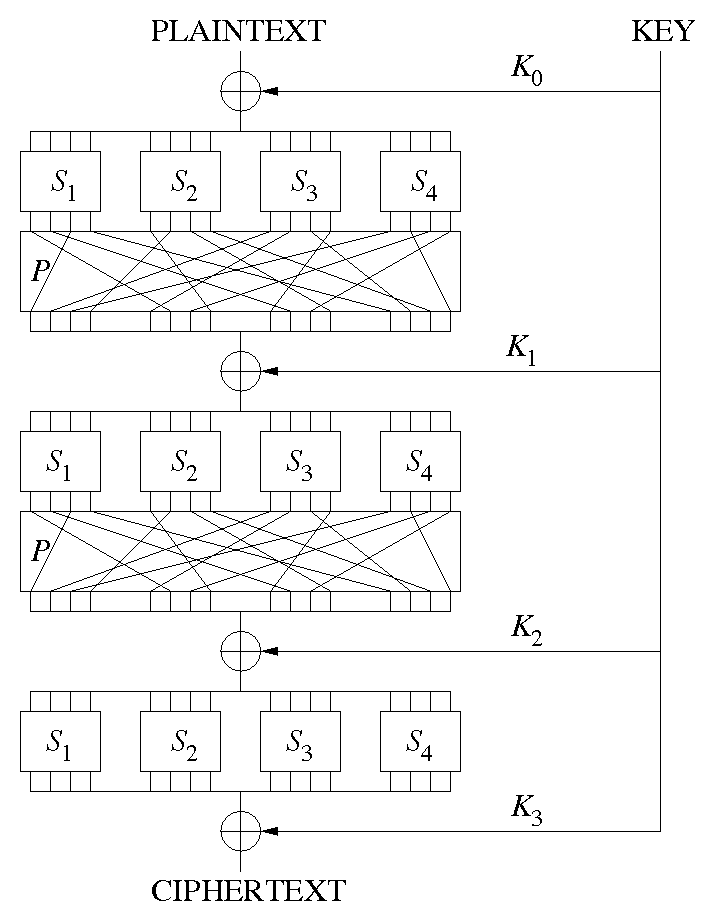
\includegraphics[width=0.5\textwidth]{../images/spn_wiki.png}
    \captionsetup{hypcap=false}
    \captionof{figure}{A sketch of a substitution–permutation network with 3 rounds, encrypting a plaintext block of 16 bits into a ciphertext block of 16 bits. The S-boxes are the Si, the P-boxes are the same P, and the round keys are the Ki. Image and caption from wikipedia.org}
    \label{fig_spn}
\end{center}
% TODO: change figure and caption (or add P box in text)

\subsubsection{AES}

The Advanced Encryption Standard (AES) is the replacement of DES chosen by the NIST in 2001.
The algorithm, also called Rijndael, is a SPN. It exists in three variants:
\begin{itemize}
    \item 10 rounds and 128-bit keys
    \item 12 rounds and 192-bit keys
    \item 14 rounds and 256-bit keys
\end{itemize}

The 128-bit block plaintext is arranged in a 4$\times$4 byte matrix
$\begin{psmallmatrix}
    m0 & m4 & m8 & m12 \\
    m1 & m5 & m9 & m13 \\
    m2 & m6 & m10 & m14 \\
    m3 & m7 & m11 & m15
\end{psmallmatrix}$
The round keys are derived using the AES key schedule.
All the 16 S-boxes are the same, and their design is chosen to have no fixed points.
The substitution operation is often referred as SubBytes operation.
The linear layer is divided into a ShiftRows and a MixColumns operation.
The ShiftRows step cyclically shifts the bytes in each row by a certain offset (from 0 to 3):
$\begin{psmallmatrix}
    m0 & m4 & m8 & m12 \\
    m1 & m5 & m9 & m13 \\
    m2 & m6 & m10 & m14 \\
    m3 & m7 & m11 & m15
\end{psmallmatrix}
\rightarrow
\begin{psmallmatrix}
    m0 & m4 & m8 & m12 \\
    m5 & m9 & m13 & m1 \\
    m10 & m14 & m2 & m6 \\
    m15 & m3 & m7 & m11 \\
\end{psmallmatrix}$


The MixColumns step then multiplies each column in place by the matrix 
$\begin{psmallmatrix}
    2 & 3 & 1 & 1 \\
    1 & 2 & 3 & 1 \\
    1 & 1 & 2 & 3 \\
    3 & 1 & 1 & 2
\end{psmallmatrix}$ so each byte of the column influences the output of the four other bytes.

The details of the AES standard are defined here \parencite{Standards2001}.

\subsection{Side Channel Analysis classic attacks}

All the implementations of cryptographic algorithms in real world devices provide more information to an attacker than just the plaintext and the ciphertext.
These side-channel leakages can consist in the timing of operations, power consumption, electromagnetic emanations, etc.
They are not taken into account by the mathematical models and very little side-channel information is enough to break many common ciphers.

Non-invasive attacks and corresponding countermeasures have been studied extensively over the past decades.

In the following, side channel attacks consist in associating the power consumption of a cryptographic module with the data processed by the module at the same time.
Indeed, the physical properties of semiconductors link the data processed by a chip to its power consumption.

To model the link between data transitions and power consumption, the Hamming weight and Hamming distance models are often used.

The \textbf{Hamming Distance} of $a \in \mathbb{F}_2^n$ and $b \in \mathbb{F}_2^n$ is $H(a \bigoplus b) = \sum_{i=0}^{n-1} \mathbbm{1}_{a_i \neq b_i}$ where $a_i$ (resp. $b_i$) is the ith bit of a (resp. b).

It counts the number of transitions when $a \rightarrow b$. For consecutive values in the same register, this metric correlates the Hamming distance with the power consumption.
However, the attacker needs to obtain consecutive data values to use this model.
A simpler solution is to consider that $a=0$. The model then becomes the following.

The \textbf{Hamming Weight} of $a \in \mathbb{F}_2^n$ is $H(a) = \sum_{i=0}^{n-1} \mathbbm{1}_{a_i = 1}$ where $a_i$ is the ith bit of a.

It counts the number of bits set to 1 when storing the variable a.
It is the most widely used leakage model.

\textbf{Single power analysis} (SPA) involves directly interpreting power consumption measurements collected during cryptographic operations \parencite{Kocher_Jaffe_Jun_1999}.
SPA can yield information about a device's operation as well as key material.

\textbf{Differential Power Analysis} (DPA) involves statistical tools to study multiple power consumption leakages from a cryptographic module.
It aims to remove noise by using signal processing and error corrections techniques.
It makes the assumption that the power consumption of a given operation follows a normal distribution at a given timestamp. 

\textbf{Correlation Power Analysis} (CPA) is similar to DPA but makes further assumptions.
It supposes a power consumption model, most often the Hamming weight model or the Hamming distance model.
It then tries to correlate the modeled power consumption with the real consumption using the Pearson correlation coefficient. % TODO: Maybe explain what the PCC is (or not)

\textbf{Template attacks} (or profiling attacks) create a profile of the attacked device with many generated traces and uses it to later find the secret of the victim with a very small number of traces.

First described in 2003, it uses a copy of the protected device to record numerous power traces using many plaintexts and keys \parencite{Chari_Rao_Rohatgi_2003}.
The noise is modeled using multivariate Gaussian distributions, one for each possible subkey.
If a subkey is a byte, then the attack would need 256 different templates.
The samples are used to identify the $n$ points where the differences between averaged signals are the largest.
These are points of interest and the model will only focus on their values.
The "templates" are then created for each subkey on these points of interest by combining the mean signal $M_i$ and the noise covariance matrix $\Sigma_{N_i}$.
The attack then consists in computing the probability that the trace from the target device originates from each one of the template.
Selecting the highest probability is optimal.
Depending on the training set, a few or even one leakage can be enough to identify a subkey.
The original paper also calculates the error probability of their test and explain how to improve the attack by pruning the least probable hypotheses.


\textbf{Mutual Information Attacks} (MIA) uses entropy and mutual information between the leakage and the predicted data.
It does not require any previous knowledge of the studied device and can be applied in any context.

The reference paper \parencite{Prouff_Rivain_2009} presents a theoretical analysis of the assumptions made in side channel attacks.
It studies MIA in the Gaussian leakage model and in the case of masked implementations.
By making fewer assumptions about the model, MIA has worse performance than other techniques using correlations between traces on devices following the Hamming weight model.
However, it could retrieve the key in a context where the trace is not linearly linked to the Hamming weight of the manipulated data.


Over the last years, \textbf{Deep Learning based Attacks} (DL) have reached the state of the art of side channel attacks.
Deep Neural Networks (DNNs) are able to efficiently break implementations of AES that resisted to other types of SCA \parencite{Maghrebi_Portigliatti_Prouff_2016}.
% TODO: explain how DNNs are useful. Or not and just conclude

These are the main side channel analysis techniques. They aim to retrieve the key, or some other secret component, involved in a known algorithm.
Template attacks even use a replica of the attacked device to "prepare" the attacks.
Nonetheless, it is also important to verify the security of cryptographic implementations against weaker opponents that do not know the exact implementation or its details.
For cryptographic systems that choose to use proprietary algorithms or a specific set of parameters for a known standard, the architecture itself is a secret component that can be determined through SCA.
The following section is about Side Channel Analysis Reverse Engineering (SCARE) and aims at assessing the gains or losses in security of choosing secret parameters for symmetric cryptography algorithms.


% \parencite{Chari_Rao_Rohatgi_2003} presents template attacks, "the strongest form of side channel attack possible in an information theoretic sense".

% \parencite{Prouff_Rivain_2009} presents the theory of Mutual Information Attacks (MIA) in side channels.

% Machine Learning is very popular right now. Thesis of \parencite{Masure}

\section{Side-Channel Analysis for Reverse Engineering}

Side-Channel Analysis for Reverse Engineering (SCARE) uses side-channel information to reverse-engineer the secret parts of a cryptographic implementation.
It applies the techniques of SCA to recover implementations details among:
\begin{itemize}
    \item Secret constants such as the substitution blocks of a SPN \parencite{Novak_2003}.
    \item Algorithm structure such as the number of rounds, the size of the S-boxes used, ...
    \item Which technologies and methods are used by the developer of the products.
\end{itemize}

\subsection{SCARE attacks on non AES ciphers}
\label{scare_non_aes}

The first SCARE attack was proposed by Novak in 2003 to retrieve the secret authentication and session key generation algorithm of the GSM standard \parencite{Novak_2003}.

The COMP128-2 algorithm used in SIM cards is kept secret despite Kerckhoffs' principle.
Knowing the architecture, the computations involved and the secret key, Novak retrieves the contents of substitution blocks implemented as lookup tables by analyzing the power consumption of the cipher.

The idea behind the attack is to use \textbf{collision analysis} because different values of a parameter can give the same intermediate result.
Identifying equal intermediate results allows an attacker to restore the content of the lookup table and thus break the substitution block.

To do that, it uses the means of measurements for all the possible values of a given input byte as an identifier.
The equality between the leakages provides a set of equation at each round of the cipher.
Combining these sets of equation allows to solve them and recover the lookup table content.

This attack is based on the assumption that two lookups to the same value gives very similar leakages.
It relies a lot on the quality of the leakages to identify identical lookups.
Because of that, \textbf{table masking} is an effective countermeasure.
It consists in decorrelating the intermediate results from the secret values.
To do that, a different random value is used each round and the operations are modified so that the final result does not depend on the random value anymore.
Implementing masking effectively is very specific to each architecture and each attacker model.
The most common masking strategies are boolean (xor $\bigoplus$) and arithmetic (+ mod $2^n$). % TODO: choose a reference for masking

\smallbreak
Another SCARE method relies on \textbf{correlation power analysis}.
An example of such attack is the reverse engineering of DES, in which the authors assume that the structure and the constants are unknown \parencite{Daudigny_Ledig_Muller_Valette_2005}.
Strong assumptions on the quality of the power leakages allow the attacker to extract scheduling information for each bit at the clock cycle level using CPA.
It means that the attacker knows exactly when each bit is manipulated.
This scheduling information from the power consumption allows the attacker to recover a good deal of information from the software implementation of DES.

Identifying patterns in power consumption and scheduling information allow to recover the general structure of the cipher: number of rounds, use of xor operation and table lookups.
For example, groups of bits manipulated together often correspond to S-box inputs.
Removing the noise and observing the scheduling information of the first round input of DES allows to recover the content of the DES expansion table line by line.
The same thing can be done for the following S-box layer and the permutation table.
The key scheduling algorithm can also be found using the same technique.

The scheduling information can then be used to isolate traces corresponding to each S-box and perform another SCA attack to recover the key.

\smallbreak
\textbf{CPA} techniques for reverse engineering can also be used under much weaker assumptions.
The attacks presented in the paper work in the known plaintext or ciphertext attacker model \parencite{Guilley_Sauvage_Micolod_Réal_Valette_2010}.
It retrieves the S-boxes of a modified DES using custom S-boxes by using brute force.
To attack $i$ input bits of a S-box, the attacker only considers a set of traces that keep 6-i bits of the target S-box to a constant value (which is possible since the plaintext is known).
A correlation program can then map these traces to the corresponding function, a subpart of the S-box.
To recover one S-box of DES, 960 CPAs are necessary using this method on 2 input bits at a time.


%\parencite{Novak_2003} presents a side-channel attack on substitution blocks with a demonstration on a SIM card using COMP-128 cipher.

%\parencite{Daudigny_Ledig_Muller_Valette_2005} presents a SCARE attack on DES and propose new methods to exploit the power measurement information.

%\parencite{Guilley_Sauvage_Micolod_Réal_Valette_20DES10} presents two SCARE attacks on the parameters of a LFSR and DES.

\subsection{SCARE attacks on AES-like ciphers}

The Advanced Encryption Standard is a publicly-known and clearly defined architecture. 
However, its parameter values can be changed to obtain a new cipher, that is not AES but has the same structure.
Following Kerckhoffs' principle, this new cipher may not be safer than a classic implementation of AES.
The following examples show how the secret parameters can be recovered using SCARE.

This SCARE method is designed for all SPN structures, including modified AES ciphers \parencite{Rivain_Roche_2013}.
It considers that the attacker can select parts of the side-channel traces where the s-box computations are located.
The attacker must be able to decide on collisions between the processed values from the observation of these traces.
For that, any SCA method can be used.
The attacker also knows the plaintext. If the plaintext is chosen, the complexity of the attack is lowered.

Then the attack consists in building simple linear equations systems to recover the S-box values, the linear layer coefficients and the secret round keys.
It retrieves the first round key by fixing its first bit and then identifying the collisions between the already known bits and the remaining bits.
Knowing the first secret round key, the collisions happening before and after the 2nd round allow to build a system of linear equations involving the linear layer, the S-box and the second secret round key.
Given enough traces, the system can be solved.
Then, only the remaining round keys are left to be discovered.
It can be done using the same method as for the first one.

This attack is very generic and can be applied to all SPNs schemes.
It also works if the leakage is noisy or on masked implementations.

According to the authors, a sufficient countermeasure is to combine masking and operation shuffling.
Non-sequential execution is also outside the scope of the attack and make it inefficient.

\smallbreak
This very general attack on SPNs has been refined for AES in 2015 under more restrictive assumptions \parencite{Clavier_Isorez_Marion_Wurcker_2015}.
The work is divided in two parts.

The first one does a SCARE of the AES under a very similar same model than Rivain and Roche \parencite{Rivain_Roche_2013}.
It still considers that the attacker can identify collisions between two different S-Box computations.
However, this method only applies to AES with secret parameters and can deal with masking and operation shuffling.
In particular, the S-box is the same for each round and the key derivation algorithm is the one from AES with secret constants.

The second part does a SCARE of the AES assuming that the attacker can identify collisions of Hamming weights of inputs/outputs of different S-box computations.
This model is weaker but more realistic.
It can resist at least to simple masking.

\smallbreak
To address the masking countermeasure, Clavier et al. only use intra-traces setting, meaning that the attacker is able to detect collisions between two S-Box only in a same execution \parencite{Clavier_Isorez_Marion_Wurcker_2015}.
Indeed, they assume that an 8-bit Boolean masking only refreshes the randomization of S-boxes at each execution because of time and memory constraints.
Then collisions that happen during one execution can be detected.
Masking on other operations do not affect the attack.

The shuffling countermeasure is more complex to evade.
It shuffles the 16 bytes S-box computations at each round, causing the collisions' observation to no longer give information about the index of the input bytes.
The remaining information is the number of different S-Box inputs at each round, and their number of occurrences.
To retrieve the first round key, it finds a plaintext such that the first round SubBytes operation only presents one colliding value occurring more than once.
By modifying each one of the 16 bytes of the plaintext and picking the indexes for which the multiplicity of the colliding value is reduced, the attacker can infer relations between the key bytes.
The process can be repeated with new plaintexts until enough relations are obtained, and the first round key can be determined (up to a xor with a constant).

The same can be done for the last round key.

To recover the S-box, the same concept is used.
Collisions between the first S-box and the last S-box computations are identified and can give information about a group of byte indexes by repeating the input bytes a different number of times for each value in a chosen plaintext.
Each collision gives information about the byte values and repeating the operation for multiple plaintexts eventually gives enough information to retrieve the S-box content.

Since the first and last round keys are known, the key scheduling algorithm can be found through exhaustive search.

To recover the ShiftRows and MixColumns parameters, the attacker can craft plaintexts by only changing one byte to obtain a small subset of possible values for MixColumns columns and ShiftRows parameters.
Different byte values provide new sets of possible values and their intersection reveals the secret parameters.

\smallbreak
To perform a SCARE attack on a modified AES under the Hamming weight model, Clavier et al. introduce and reason on special sets.
They are constituted of the inputs (respectively the outputs) that have a given Hamming weight and whose S-box output (respectively input) has another given Hamming weight that will collide under the Hamming weight collisions model.
The attack first retrieves the first and last round keys and the ShiftRow parameters, then builds the special sets by analyzing collisions and non-collisions between chosen plaintexts, and reasons on their cardinal.
The special sets allow to reduce the number of potential candidates for each byte value during the MixColumns and S-box retrieval stages.
If a set has a cardinal of 1, then it identifies one unique value.

This attack is very efficient and can recover the parameters of an AES using approximately 250 traces, whereas 400 (respectively 4000) are needed under the unprotected (respectively protected by a first-order Boolean masking and a random shuffling of operations) collision value model.


% Est-ce vraimentpertinent de parler d'une cryptanalyse dans un rapport sur les SCA ?
%\parencite{Tiessen_Knudsen_Kölbl_Lauridsen_2015} presents an integral cryptanalysis of an AES with a secret S-box and fewer rounds. It is not a SCA but is still closely related to our subject.

%\parencite{Rivain_Roche_2013} presents a generic SCARE attack against a wide class of SPN block ciphers.

%FIRE (injection fault attempts) and SCARE attacks to recover the full set of secret parameters of an AES-like software implementation, even with masking and shuffling \parencite{Clavier_Isorez_Marion_Wurcker_2015}.

\section{Application to hardware implementations}

\subsection{Differences between software and hardware cryptographic implementations}

Software implementations are exposed to illegitimate access to their machine code through memory dumping.
This can often be done without damaging the component.
Because of that, it is more secure to implement the cryptographic algorithm into a specific device.
It allows for better performances and better security through isolation of the component.

Also, implementing cryptography in hardware modules makes it more difficult to use SCA techniques.
Indeed, many SCA attacks assume that the execution is sequential, whereas cryptographic modules implemented on an ASIC or an FPGA use parallelization whenever it is possible.
Parallelizing the S-box lookups makes it impossible to get clean and separated power consumption traces.

Then, hardware cryptographic implementations leakages are noisier, due to the physical setup and can use other countermeasures, such as desynchronized execution.
So attacks on hardware devices cannot recover as much information as attacks on software algorithms.
For example, the precise scheduling information recovered in the attack presented in \ref{scare_non_aes} is unrealistic on a hardware target \parencite{Daudigny_Ledig_Muller_Valette_2005}.


Due to the higher cost of developing, evaluating and attacking hardware cryptographic implementations, and the lack of reproducibility of the studies due to different experimental setups (acquisition platform sensitivity, cryptographic algorithm implementation, board's noise), the literature on the subject is scarcer.

To address the lack of uniformized benchmark, the DPA Contest v2 proposed in 2010 a common framework for multiple team to compare their attacks \parencite{Clavier_Danger_Duc_Elaabid_Gérard_Guilley_Heuser_Kasper_Li_Lomné_et_al_2014}.
The target is an FPGA implementation of an AES-128, and it considers known-message and profiled attacks.
The acquisition board and its setup are precisely defined, and many metrics are used to evaluate the attacks: partial success rate, partial guessing entropy, global success rate, execution time and memory footprint.

The results of the contest emphasize many differences between software side channel analysis and hardware side channel analysis.
An example is the higher inaccuracy of the models such as the Hamming distance model used to approximate the traces.
This inaccuracy makes classical attacks adaptation more difficult but also allows new opportunities of improve them.

% \begin{itemize}
%     \item The sequential execution becomes parallel
%     \item There is even more noise
%     \item SCA leaks cannot be determined as precisely
%     \item It takes more time to implement, develop and attack
% \end{itemize}

% \parencite{Clavier_Danger_Duc_Elaabid_Gérard_Guilley_Heuser_Kasper_Li_Lomné_et_al_2014} presents the result of the DPA contest.

\subsection{Attacks on hardware design}

\parencite{Réal_Dubois_Guilloux_Valette_Drissi_2008} presents a SCARE attack on a general Feistel scheme with an hardware design.

SAKURA board reference

\parencite{Guilley_Sauvage_Micolod_Réal_Valette_2010} presents two SCARE attacks on the parameters of a LFSR and DES, implemented on FPGAs.

SCA attacks on FPGAs (\parencite{Peeters_Standaert_Donckers_Quisquater_2005} or more relevantly \parencite{Standaert_Ors_Preneel_2004} or something more recent)


\section{Conclusion}

\section*{References}

\printbibliography

\end{document}
%%% Local Variables:
%%% mode: latex
%%% TeX-master: t
%%% End: